\documentclass{article}

% Packages for special characters and symbols
\usepackage[utf8]{inputenc}
\usepackage[T1]{fontenc}
\usepackage{amsmath, amssymb, amsthm}

% Package for hyperlinks
\usepackage{hyperref}

% Package for graphics
\usepackage{graphicx}
\usepackage{listings}
\usepackage{dirtree}

% Package for better tables
\usepackage{booktabs}
\usepackage{xepersian}

% \setlatintextfont{Times New Roman}
\settextfont{Yas.ttf}
% Set the title, author, and date
\title{گزارش پروژه اول علوم اعصاب محاسباتی}
\author{امیرحسین انتظاری}
\date{\today}

% Begin document
\begin{document}

% Create the title
\maketitle
\newpage
% Create a table of contents
% \tableofcontents
% Separate the table of contents from the next content with a new page
% \clearpage

    \begin{abstract}
        در این پروژه، قصد داریم که مدل مدل های نورونی تجمیع و آتش نشتی
        ($LIF$)، 
        تجمیع و آتش نشتی نمایی
        ($ELIF$)و 
        تجمیع و آتش نشتی نمایی و تطبیق پذیر
        ($AELIF$) 
        را با استفاده از زبان پایتون و کتابخانه 
        $PymoNNtorch$ 
        و به روش اویلر پیاده سازی کنیم. سپس عملکرد هر یک از این مدل ها را با استفاده از جریان های متفاوت مورد بررسی قرار می دهیم و با ارائه نمودار های مختلف، عملکرد آن ها را تحلیل میکنیم. همچنین این مدل ها را با اضافه کردن نویز به جریان های متفاوت آزمایش میکنیم تا رفتار آن ها را نسبت به نویز بسنجیم. همچنین اضافه کردن بازه مقاومت
        ($Refractory$)
        به مدل ها شبیه سازی میکنیم. در نهایت نیز مدل ها را با پارامتر های متفاوت آزمایش میکنیم تا تاثیر هر یک از پارامتر ها بر مدل را بهتر لمس کنیم.
    \end{abstract}

\newpage
    \section{پیاده سازی}
    \subsection{کتابخانه ها}
        برای پیاده سازی این پروژه، به طور کلی از کتابخانه های
        $PymoNNtorch$، 
        $matplotlib$ 
        استفاده کردم که کتابخانه 
        $PymoNNtorch$ 
        برای ساخت مدل ها و کتابخانه 
        $matplotlib$ 
        برای کشیدن نمودار ها استفاده شد.
        کتابخانه
        $PymoNNtorch$ 
        توسط تیم آزمایشگاه علوم اعصاب محاسباتی دانشگاه تهران بر پایه 
        $PymoNNto$ و
        $torch$ 
        توسعه داده شده است.

    \subsection{مقدمه ای بر کتابخانه \text{PymoNNtorch}}
        برای این پروژه، ما به سه ماژول کلی از این کتابخانه نیاز داریم: ماژول شبکه
        ($Network$)، 
        گروه نورونی
        ($NeuronGroup$) و
        رفتار 
        ($Behavior$).

        کلاس 
        \textbf{$Network$} 
        برای ساخت یک شبکه عصبی است. این کلاس نگهدارنده تمام مولفه های شبکه عصبی است که باید شبیه سازی شوند. تمام اشیا یک مصداق 
        ($instance$) 
        از این کلاس را دریافت می کنند.\cite{PymoNNtorch}

        کلاس 
        \textbf{$NeuronGroup$}
        برای تعریف گروهی از نورون ها استفاده می شود. این کلاس علاوه بر پارامتر شبکه 
        ($net$)،
        پارامتر های اندازه
        ($size$)، 
        برای تعیین تعداد نورون ها و پارامتر رفتار
        ($behavior$) 
        برای اعمال رفتار های مورد نظر را دریافت می کند. البته پارامتر های دیگری نیز می گیرد که در این پروژه مورد نیاز نبودند.

        کلاس 
        \textbf{$Behavior$}
        هسته اصلی ایده های مورد استفاده در پروژه ما می باشد و نیاز به توضیح بیشتری دارد. در واقع اینطور که من متوجه شدم، کلاس اشیای اصلی که ما در این پروژه استفاده میکنیم، یک ورودی به صورت دیکشنری که شامل چندین کلاس ارث بری شده از 
        $Behavior$ 
        هستند را دریافت میکنند و قابلیت اعمال آن را روی خود دارند.
        مثلا، کلاس شبکه
        ($Network$) 
        میتواند یک سری رفتار را دریافت کند و آن را روی همه کلاس هایی که بر بستر آن هستند، اعمال کند. به طور بخصوص در این پروژه، رفتاری که روی شبکه ها اعمال شد، دقت زمانی
        ($TimeResolution$) 
        بود. یا به عنوان مثال دیگر، مدل تجمیع و آتش نشتی
        ($LIF$) 
        تحت عنوان یک رفتار روی یک گروهی نورونی می تواند اعمال شود.

        \subsection{تعریف یک رفتار}
            حال به طور دقیق تر به این موضوع می پردازیم که چگونه می توان یک رفتار را تعریف کرد. به طور خاص، تعریف رفتار ها برای یک گروه نورونی را در نظر میگیریم. گفتیم که یک مصداق از کلاس
            $NeuronGroup$، 
            رفتار ها را به صورت یک دیکشنری دریافت می کند. کلیدها در این دیکشنری، به صورت اعداد هستند که ترتیب اعمال رفتار در گروهی نورونی ما هستند.
            
            برای تعریف یک رفتار، نیاز داریم که یک کلاس تعریف کرده که از کلاس 
            $Behavior$ 
            ارث بری کند.
            این کلاس دو تابع 
            \texttt{initialize} و
            \texttt{forward} 
            را در اختیار ما قرار می دهد.
            \begin{itemize}
                \item \texttt{initialize}:
                در این تابع، پارامتر های رفتار تعریف می شوند و مقادیر اولیه آن ها قرار داده می شود. اینکار توسط تابع 
                \texttt{self.parameter} 
                انجام می شود. اگر نیاز به تعریف متغیر اضافه ای در گروه نورونی باشد نیز، در این تابع تعریف می شود.
                \item \texttt{forward}:
                در این تابع، عملیات هایی که لازم است که در هر تکرار شبیه سازی انجام شود، تعریف می شوند.
            \end{itemize}
            با ارائه یک مثال از تعریف یک رفتار مانند مدل تجمیع و آتش نشتی
            ($LIF$) 
            تعریف را دقیق تر می کنیم.
        \begin{latin}        
            \centering        
                \begin{lstlisting}[language=Python]
class LIF(Behavior):
    def initialize(self, ng):
        # initial parameters in LIF model
        self.R = self.parameter("R", None, required=True)
        self.tau = self.parameter("tau", None, required=True)
        self.u_rest = self.parameter("u_rest", None, required=True)
        self.u_reset = self.parameter("u_reset", None, required=True)
        self.threshold = self.parameter("threshold", None, required=True)
        # initial value of u in neurons
        ng.u = ng.vector(0) 
        ng.u += self.u_reset
        ng.spike = ng.u > self.threshold
        ng.u[ng.spike] = self.u_reset


    def forward(self, ng):
        # Neuron dynamic
        inp_u = self.R * ng.I 
        leakage = ng.u - self.u_rest
        ng.u += ((-leakage + inp_u) / self.tau) * ng.network.dt
        # Firing
        ng.spike = ng.u > self.threshold
        # Reset
        ng.u[ng.spike] = self.u_reset
            \end{lstlisting}
        \end{latin}
            
            می دانیم که دینامیک مدل نورونی تجمیع و آتش نشتی، 
            ($LIF$) 
            به صورت زیر است:
            \begin{latin}
                \begin{equation}
                    \tau.\frac{du}{dt}=-(u-u_{rest}) + R.I(t); \text{if firing:} (u=u_{rest})
                \end{equation}
            \end{latin}
            که ما میتوانیم ولتاژ لحظه بعدی را با استفاده از داشتن ولتاژ قبلی و جمع کردن آن با 
            $du$ 
            بدست بیاوریم، پس معادله را میتوان به صورت زیر باز نویسی میکنیم:
            \begin{latin}
                \begin{equation}\label{eqn:lif-du}
                    du=\frac{(-(u-u_{rest}) + R.I(t))\times dt}{\tau}
                \end{equation}
            \end{latin}
            حال میخواهیم ببینیم چگونه می توان این دینامیک را پیاده سازی کرد. در ابتدا نیاز داریم که متغیر ها و پارامتر های مورد نیاز را تعریف کنیم. این پارامتر ها عبارتند از 
            $R$,
            $tau$,
            $u_{rest}$,
            $u_{reset}$,
            آستانه
            ($threshold$).
            اینکار با استفاده از تابع 
            \texttt{self.parameter()} 
            قابل انجام است که در آن می توان مقدار پیش فرض و همچنین ضروری بودن آن را تنظیم کرد. برای اکثر متغیر ها بهتر است مقدار پیش فرض به 
            \texttt{None} 
            مقدار دهی شود و ضروری بودن آن نیز درست
            \texttt{True} 
            باشد.

            پس از تعریف پارامتر ها، متغیر های مورد نیاز مانند ولتاژ
            ($u$)
            یا لحظه ضربه
            ($spike$)
            زدن
            را برای نورون ها مقدار دهی میکنیم.(به صورت یک آرایه به اندازه تعداد نورون ها)

            حال نوبت به تعریف تابع 
            \texttt{forward} 
            می رسد. اینجا همانجایی است که شبیه سازی ما انجام می شود.
            برای اینکار، کافی است معادله
            \ref{eqn:lif-du}
            را به صورت کد نوشته و با 
            \texttt{ng.u} 
            جمع کنیم. پس از آن نیز، اگر نورونی از آستانه گذشت، مقدار آن در آرایه
            ($tensor$) 
            \texttt{ng.spike} 
            را 
            \texttt{True} 
            می کنیم.

            اینکار را می توان به طور مشابه برای بقیه مدل های نورونی، یعنی مدل تجمیع و آتش نشتی نمایی
            ($ELIF$) 
            و مدل تجمیع و آتش نشتی نمایی تطبیق پذیر
            ($AELIF$) 
            یا حتی رفتار هایی مانند جریان یا نویز یا موارد دلخواه دیگر را نیز انجام داد و اگر پارامتر یا متغیر اضافه ای نیاز بود، اضافه کرد.
    

        \subsection{توضیحات تکمیلی}
            برای این پروژه سعی من این بود که تا حد امکان، علاوه بر انجام دادن وظایف مورد انتظار، بتوانم توابع را به گونه ای تعریف کنم که ماژولار بوده و بتوان دوباره نیز از آن ها استفاده کرد. همچنین نحوه ساخت فایل ها به گونه ای بود که هم ساختار درستی داشته باشند و هم اشیا و توابع مرتبط در یک فایل باشند تا بتوان در نهایت از آن ها در یک فایل 
            $nootbook$ 
            استفاده کرد.
            درخت کلی فایل های پروژه به صورت زیر می باشد:
            \dirtree{%
            .1 code.
            .2 aelif\_main.py.
            .2 currents.py.
            .2 elif\_main.py.
            .2 main.ipynb.
            .2 models.py.
            .2 plots.py.
            .2 simulate.py.
            .2 time\_res.py.
            }
            در فایل 
            \texttt{models.py}
            کلاس مدل های نورونی وجود دارند. به طور مشابه، کلاس مدل های جریان و دقت زمانی نیز به ترتیب در 
            \texttt{currents.py} و
            \texttt{time\_res.py} 
            قرار دارند.
            در هر یک از فایل های 
            \texttt{lif\_main.py}، 
            \texttt{elif\_main.py} و 
            \texttt{aelif\_main.py}
            نیز یک شبکه ساده و یک نمودار برای آزمایش کردن مدل ها هنگام توسعه کد نوشته شده است.
            کد های اضافه اینجانب مانند کد های شبیه سازی و کشیدن نمودار های مختلف نیز به ترتیب در 
            \texttt{simulate.py} و
            \texttt{plots.py} 
            قرار دارند. هر چند در فرایند توسعه کد ها، کلاس
            \texttt{Simulation} 
            به تنهایی مجهز به نمایش نمودار ها نیز شد ولی در صورت نیاز میتوان از نمودار های فایل 
            \texttt{plots.py} 
            نیز استفاده نمود.
            علاوه بر این موارد، سعی شده تا کد ها از قوانین 
            $clean\text{ }code$ 
            پایتون مانند 
            $PEP8$ 
            استفاده و رعایت شوند.

            شایان ذکر است که تمام روند توسعه پروژه بر بستر کنترل نسخه 
            $Git$ 
            انجام شد تا در صورت نیاز، بتوان از آن ها در پروژه های آینده نیز استفاده کرد.

\newpage
    \section{شبیه سازی مدل ها با جریان های مختلف}
        در این قسمت پروژه، مدل های پیاده سازی شده را، با جریان های مختلف پیاده سازی میکنیم. من علاوه بر سه جریان اصلی گفته شده در پروژه، یعنی جریان ثابت، جریان پله و جریان سینوسی، دو جریان تابع شیب دار ساده و تابع لگاریتمی را نیز بررسی کردم. هر چند توابع دیگری مانند تابع نمایی نیز ممکن است به ذهن برای شبیه سازی خطور کند اما در عمل این تابع جالب نمی باشد چرا که فرض کردن تغییر جریان به صورت نمایی درست به نظر نمی رسد و همچنین پیاده سازی آن، بعد از چند لحظه کوتاه، منجر به ضربه 
        ($spike$) 
        های ممتد با فواصل بسیار کم می شود. 
        
        در ادامه نمودار های خواسته شده را برای مدل های گفته شده تحلیل و بررسی میکنیم.

        \subsection{مدل تجمیع و آتش نشتی ($LIF$)}
            \subsubsection{جریان ثابت}
            اولین نمودار
            (شکل \ref{fig:lif-const-curr})
            مربوط به مدل تجمیع و آتش نشتی
            ($LIF$) 
            با جریان ثابت است. در این مدل جریان ورودی برابر با 
            $10$، 
            مقاومت برابر با 
            $5$ ، 
            $\tau$ 
            برابر با 
            $10$،  
            آستانه($threshold$) 
            برابر با 
            $-37$ 
            و اختلاف پتانسیل استراحت و ریست
            ($reset$) 
            به ترتیب برابر با 
            $-67$ و
            $-75$ 
            می باشند. همانطور که ملاحظه می شود، از آنجا که جریان ورودی به نورون ثابت می باشد، اختلاف پتانسیل غشای نورون در ابتدا به تدریج بالا رفته و زمانی که به آستانه خود می رسد، یک ضربه
            ($spike$) 
            میزند. پس از زدن ضربه نیز، از آنجا که افزایش ناگهانی اختلاف پتانسیل در مدل تجمیع و آتش نشتی ساده، شبیه سازی نمی شود، به طور دستی ناگهان برابر با اختلاف پتانسیل ریست
            $reset$ 
            می شود.

            \begin{figure}[h]
                \centering
                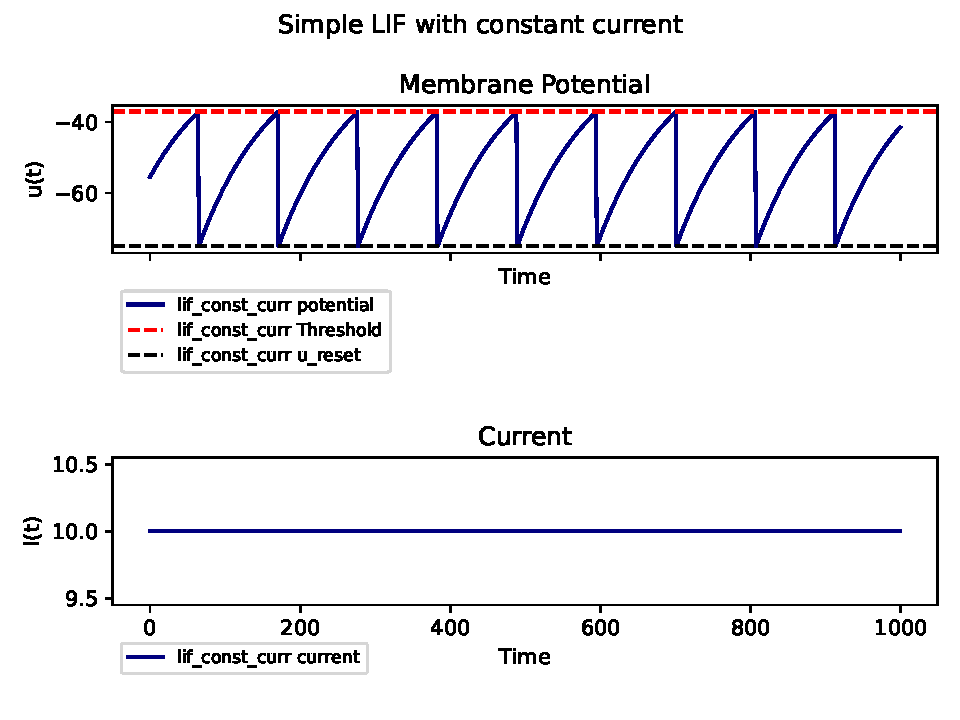
\includegraphics[width=0.8\textwidth]{plots/Simple LIF with constant current.pdf} % Include the exported plot
                \caption{مدل تجمیع و آتش نشتی با جریان ثابت.}
                \label{fig:lif-const-curr}
            \end{figure}

            حال بیاییم برخی پارامتر های مدلمان را تغییر دهیم تا تاثیر آن ها را مشاهده کنیم. اینکار را برای سه جریان متفاوت خیلی کم، کم و زیاد آزمایش میکنیم. همانطور که در نمودار 
            \ref{fig:lif-const-change-current-curr} 
            ملاحظه میکنید، با افزایش جریان، فرکانس ضربه ها
            ($spike$)
            بیشتر می شود و فواصل بین آن ها کم می شود.(منحنی قرمز)
            به طور عکس، کاهش کم جریان، میتواند تاثیر عکس داشته و فواصل بین ضربه ها را بیشتر کند.
            همچنین کاهش زیاد جریان سبب می شود که نورون به آستانه خود نرسد و هیچگاه ضربه نزند. این موضوع می تواند زمان استراحت نورون را که ورودی ای ندارد را توجیه کند.

            \begin{figure}[h]
                \centering
                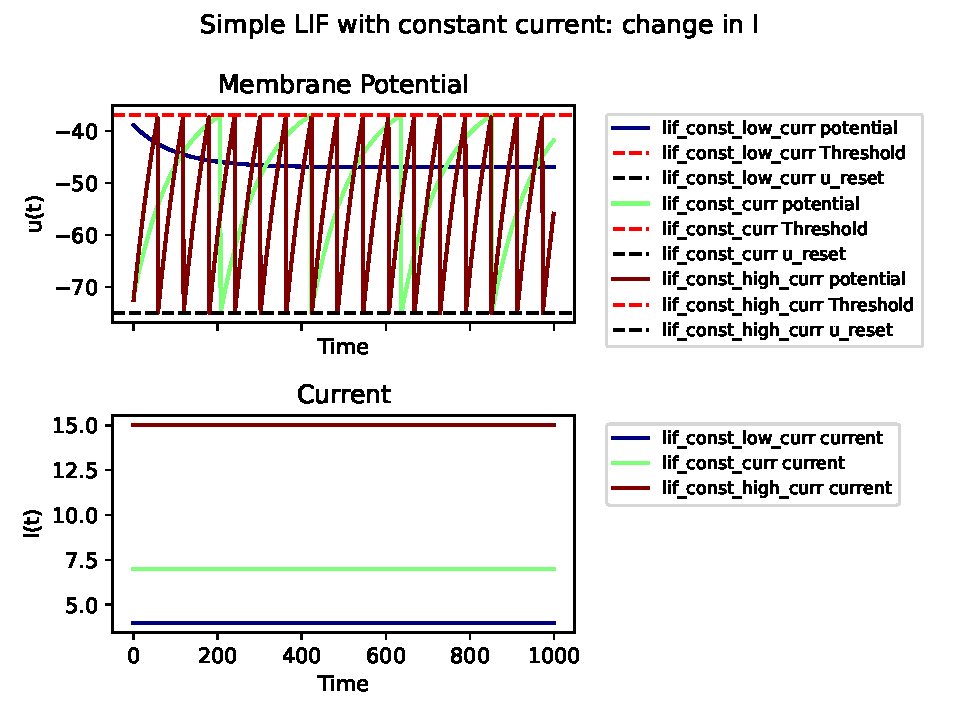
\includegraphics[width=0.8\textwidth]{plots/Simple LIF with constant current: change in I.pdf} 
                \caption{مدل تجمیع و آتش نشتی با جریان ثابت: تغییر در جریان}
                \label{fig:lif-const-change-current-curr}
            \end{figure}

            از آنجا که مدل تجمیع و آتش نشتی ساده است، تغییر پارامتر های دیگر تاثیر مشابه داشته و تنها فرکانس ضربه ها را تغییر می دهد. به طور مثال، کاهش/افزایش آستانه می تواند باعث افزایش/کاهش فرکانس ضربه ها شود.(به طور مشابه برای دیگر پارامتر ها)

            \subsubsection{جریان پله ای}
                جریان بعدی، از تابع پله ای پیروی میکند. در تابع پله ای، جریان در لحظه ای وصل شده و پس از مدت زمانی قطع می شود. پارامتر های این نمودار، کاملا مشابه جریان ثابت داده شده است و فقط در لحظات ۲۵۰ و ۷۵۰، جریان ثابت متصل می شود. در مدل تجمیع و آتش نشتی
                ($LIF$)
                لحظاتی که جریان وصل است، اختلاف پتانسیل غشای نورون مانند جریان ثابت عمل می کند. از این رو برای ما، لحظاتی که جریان وصل و قطع می شود جذاب است. همانطور که در شکل 
                \ref{fig:lif-step-curr} 
                مشاهده می شود، در ابتدای شبیه سازی، از آنجا که جریان اولیه نورون به صورت تصادفی مقدار دهی می شود، ما مقدار در حدود 
                $-65$ 
                داریم که از پتانسیل استراحت بیشتر است، پس این اختلاف پتانسیل کم کم به سمت پتانسیل استراحت یعنی 
                $-67$ 
                حرکت می کند. در لحظه ۲۵۰، جریان ثابت به نورون متصل می شود و همانطور که از نمودار پیداست، اختلاف پتانسیل غشای نورون رفته رفته بیشتر می شود تا در نهایت یک ضربه
                ($spike$)
                می زند. از این لحظه تا لحظه  ۷۵۰، رفتار نورون کاملا شبیه حالت قبل یعنی جریان ثابت می باشد. از لحظه ۷۵۰ که جریان قطع می شود، اختلاف پتانسیل نورون که تازه ضربه زده بوده و بالا می باشد، به سمت پتانسیل استراحت حرکت می کند.
                \begin{figure}[h]
                    \centering
                    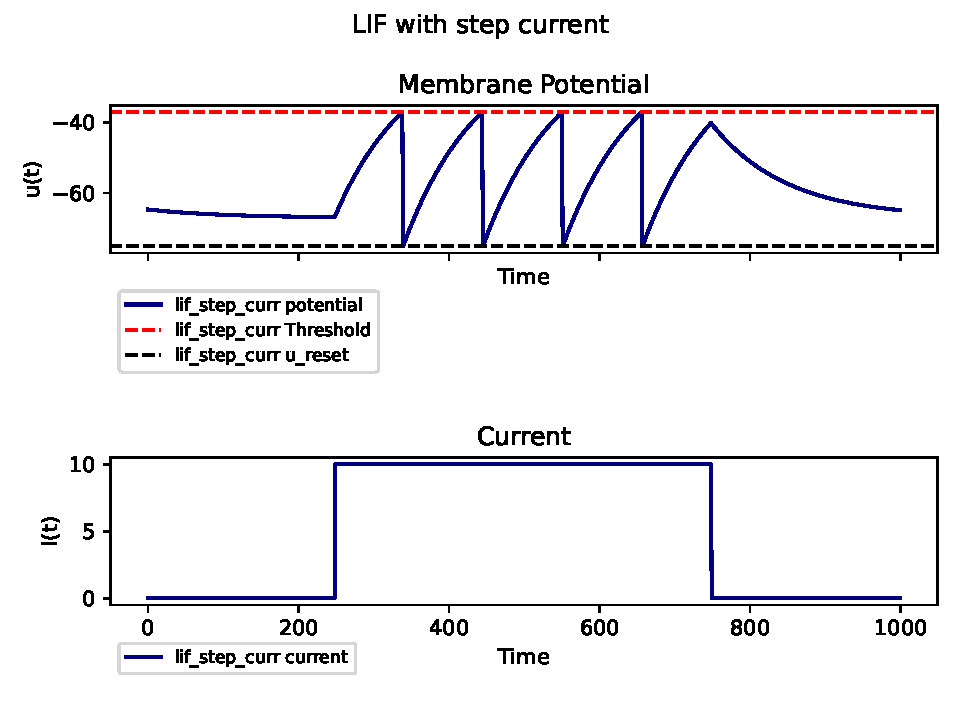
\includegraphics[width=0.8\textwidth]{plots/LIF with step current.pdf} 
                    \caption{مدل تجمیع و آتش نشتی با جریان پله ای}
                    \label{fig:lif-step-curr}
                \end{figure}
                واضح است که آزمایش این مدل با جریان پله ای و پارامتر های مختلف، نتیجه ای مشابه با جریان ثابت خواهد داشت.

            \subsubsection{جریان سینوسی}
                حال به بررسی رفتار نورون با مدل تجمیع و آتش نشتی ساده با جریان سینوسی می پردازیم. پارامتر های مدل 
                $LIF$
                مان اینجا نیز مانند قبل داده شده است.
                برای شبیه سازی جریان به صورت سینوسی نیز، از کلاس 
                \texttt{SinCurrent} 
                استفاده شده است که در آن، پارامتر های تعداد فرکانس
                ($frequency$) 
                دامنه نوسان
                ($amplitude$)
                و جابه جایی عمودی و افقی داده شده است. این پارامتر ها در نمودار زیر، به ترتیب با اعداد 
                $20$, 
                $2$, 
                $2$ و
                $10$ 
                داده شده است.
                از این رو، جریان بین 
                $-10$ و
                $30$ 
                نوسان می کند. 
                \begin{figure}[h]
                    \centering
                    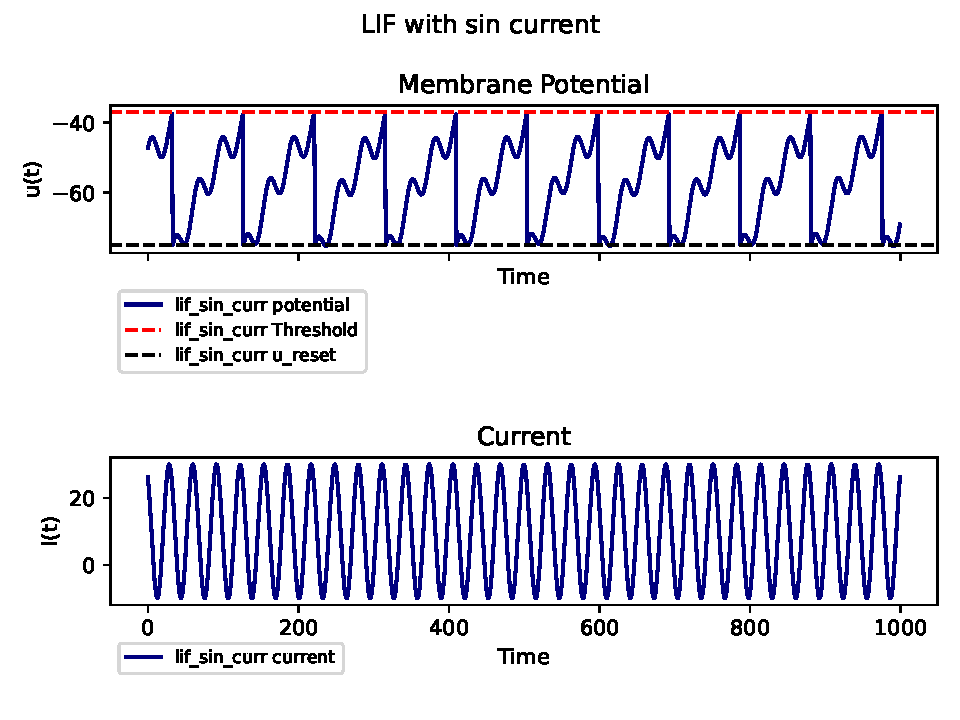
\includegraphics[width=0.8\textwidth]{plots/LIF with sin current.pdf} 
                    \caption{مدل تجمیع و آتش نشتی با جریان سینوسی}
                    \label{fig:lif-sin-curr}
                \end{figure}



% Start a new section
\newpage
\section{مدل}

This is the methodology section of your article.



% Bibliography section
\newpage
\begin{thebibliography}{1}
    \bibitem{textbook}
        \begin{latin}
            Computational Neuroscience Course, School of computer science, University of Tehran
        \end{latin}
    \bibitem{PymoNNtorch}
        \begin{latin}
            PymoNNtorchPytorch-adapted version of PymoNNto
        \end{latin}
    
    \end{thebibliography}
\end{document}
